

\chapter{System Operations}
\label{sec:System Operations}

In the context of this system and \ac{an} state calculation, the basic operations to determine the state of a neuron is to :
\begin{outline}
    \1 Synchronization to other managers
    \1 Inform the Manager and \ac{pe} which operations are to be performed
    \1 Inform the manager where to access the states of the pre-synaptic neurons
    \1 Inform the manager where to access the weights of the connections from the pre-synaptic ANs
    \1 How to provide the pre-synaptic neuron weights and states to the processing engine execution lanes
    \1 Inform the manager where to store the resulting AN state back to memory
\end{outline}


This work has developed an instruction architecture to describe the above operations.
In the baseline system, the manager is not responsible for performing specific algorithm computational operations but is responsible for coordinating the various data flows and configuration of the modules that make up the system.

The managers primary responsibility is:

\begin{outline}
    \1 System Control
    \1 Instruction decode
    \1 Internal Configuration messages
    \1 Operand read
    \1 Result write
    \1 Inter-manager communication
\end{outline}

In the baseline system, the \ac{pe} is responsible for the main algorithm operations.

The \ac{pe} has three major blocks:

\begin{outline}
  %\setlength{\baselineskip}{10pt}
  %\setlength{\itemsep}{6pt}
    \1 Streaming operation function (\ac{stop})
      \2 Processes data from the manager on-the-fly without storing in local \ac{sram}
    \1 \ac{simd}
      \2 processes the data from the \ac{stop} before returning data to the manager
    \1 DMA/local memory controller
      \2 transfer configuration data to \ac{pe} controller or to store \ac{stop} results to a small local \ac{sram} which can be used for access by \ac{simd} or by the \ac{stop} function
\end{outline}
% ----------------------------------------------------------------------------------------------------
% ----------------------------------------------------------------------------------------------------
\section{Manager Operations}
\label{sec:Manager Operations}

% ----------------------------------------------------------------------------------------------------
\subsection{Instructions}
\label{sec:Instructions}
The instructions include information to control the operations below:

\begin{outline}
  %\setlength{\baselineskip}{10pt}
  %\setlength{\itemsep}{6pt}
  %\setlength{\baselineskip}{10pt}
  %\setlength\itemsep{0pt}
  %\setlength{\partopsep}{0pt}
  %\setlength{\parskip}{0pt}
  %\setlength{\parsep}{0pt}
  %\setlength{\topsep}{0pt}
  %\setlength{\itemsep}{3pt}
  %\setlength{\itemindent}{\leftmargin}
  %\setlength{\leftmargin}{0pt}
        \1 To the Manager
            \2 Operation descriptor
            \2 Parameter/Weight Storage Descriptor(s)
                \3 reads for the two argument streams to the \ac{pe}
                \3 read data can be broadcast or vectored to the \ac{pe}
            \2 Result write storage descriptor
                \3 include descriptors for all destination managers
            \2 Synchronization to other managers
        \1 To the \ac{pe}
            \2 \ac{stop} operation
            \2 \ac{simd} operation
            \2 Number of active lanes
            \2 Operand Vector length
\end{outline}


Instructions contain sub-instructions called descriptors. These descriptors contain, amongst other things the information to control the various operations associated with the processing of a group of \acp{an}.
The size of this group of \acp{an} is related to the number of execution lanes, which for this work is 32. A group can be anywhere from 1-32. It should be said that unless the group size consistently approaches 32 the system performance will be poor.

To perform \ac{an} activation calculations, an instruction will typically have four descriptors which will include:

\begin{outline}
\renewcommand{\outlinei}{enumerate}
    \1 Operation descriptor 
    \1 Memory read descriptor for operand stream 0
    \1 Memory read descriptor for operand stream 1
    \1 Result descriptor write
\end{outline}

The instruction is an n-tuple where the tuple elements are descriptors. The number of descriptors can vary based on the operation being performed. 
In figure \ref{fig:Instruction (4-tuple example)} we see the format of a 4-tuple instruction which is used to perform an activation calculation for a group of \acp{an}.

\begin{figure}[!t]
\centering
\captionsetup{justification=centering}
\captionsetup{width=.9\linewidth}
\centerline{
\mbox{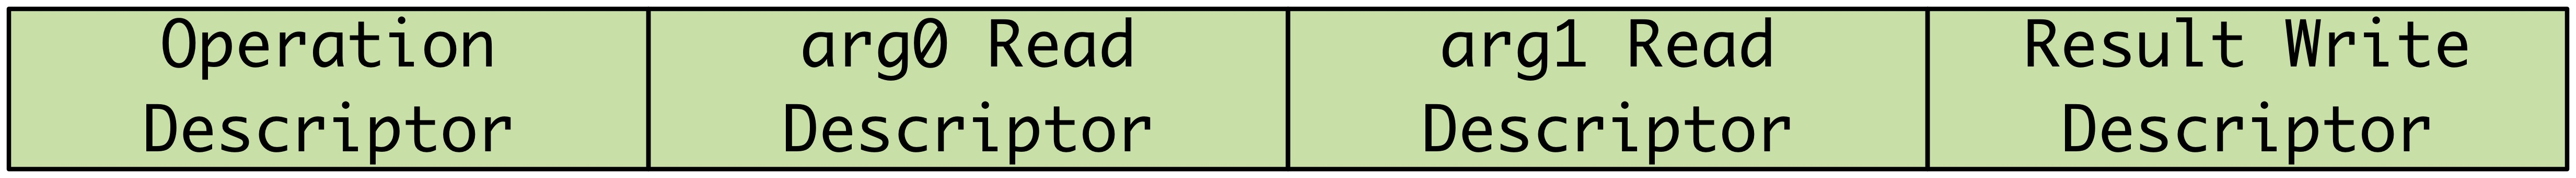
\includegraphics[width=.9\linewidth]{instruction4Tuple.jpg}}
}
\caption{Instruction (4-tuple example)}
\label{fig:Instruction (4-tuple example)}
\end{figure}

Within a descriptor, various options are described, such as storage descriptor pointer, number of operands etc..
The descriptor also employs an n-tuple format where the first tuple element always describes the descriptor operation followed by an m-tuple whose elements contain the options required by the operation.
The option elements within a descriptor are a two-tuple with option and associated value.
In figure \ref{fig:descriptorTuple} we see the format of a 6-tuple descriptor.

\begin{figure}[!t]
\centering
\captionsetup{justification=centering}
\captionsetup{width=.9\linewidth}
\centerline{
\mbox{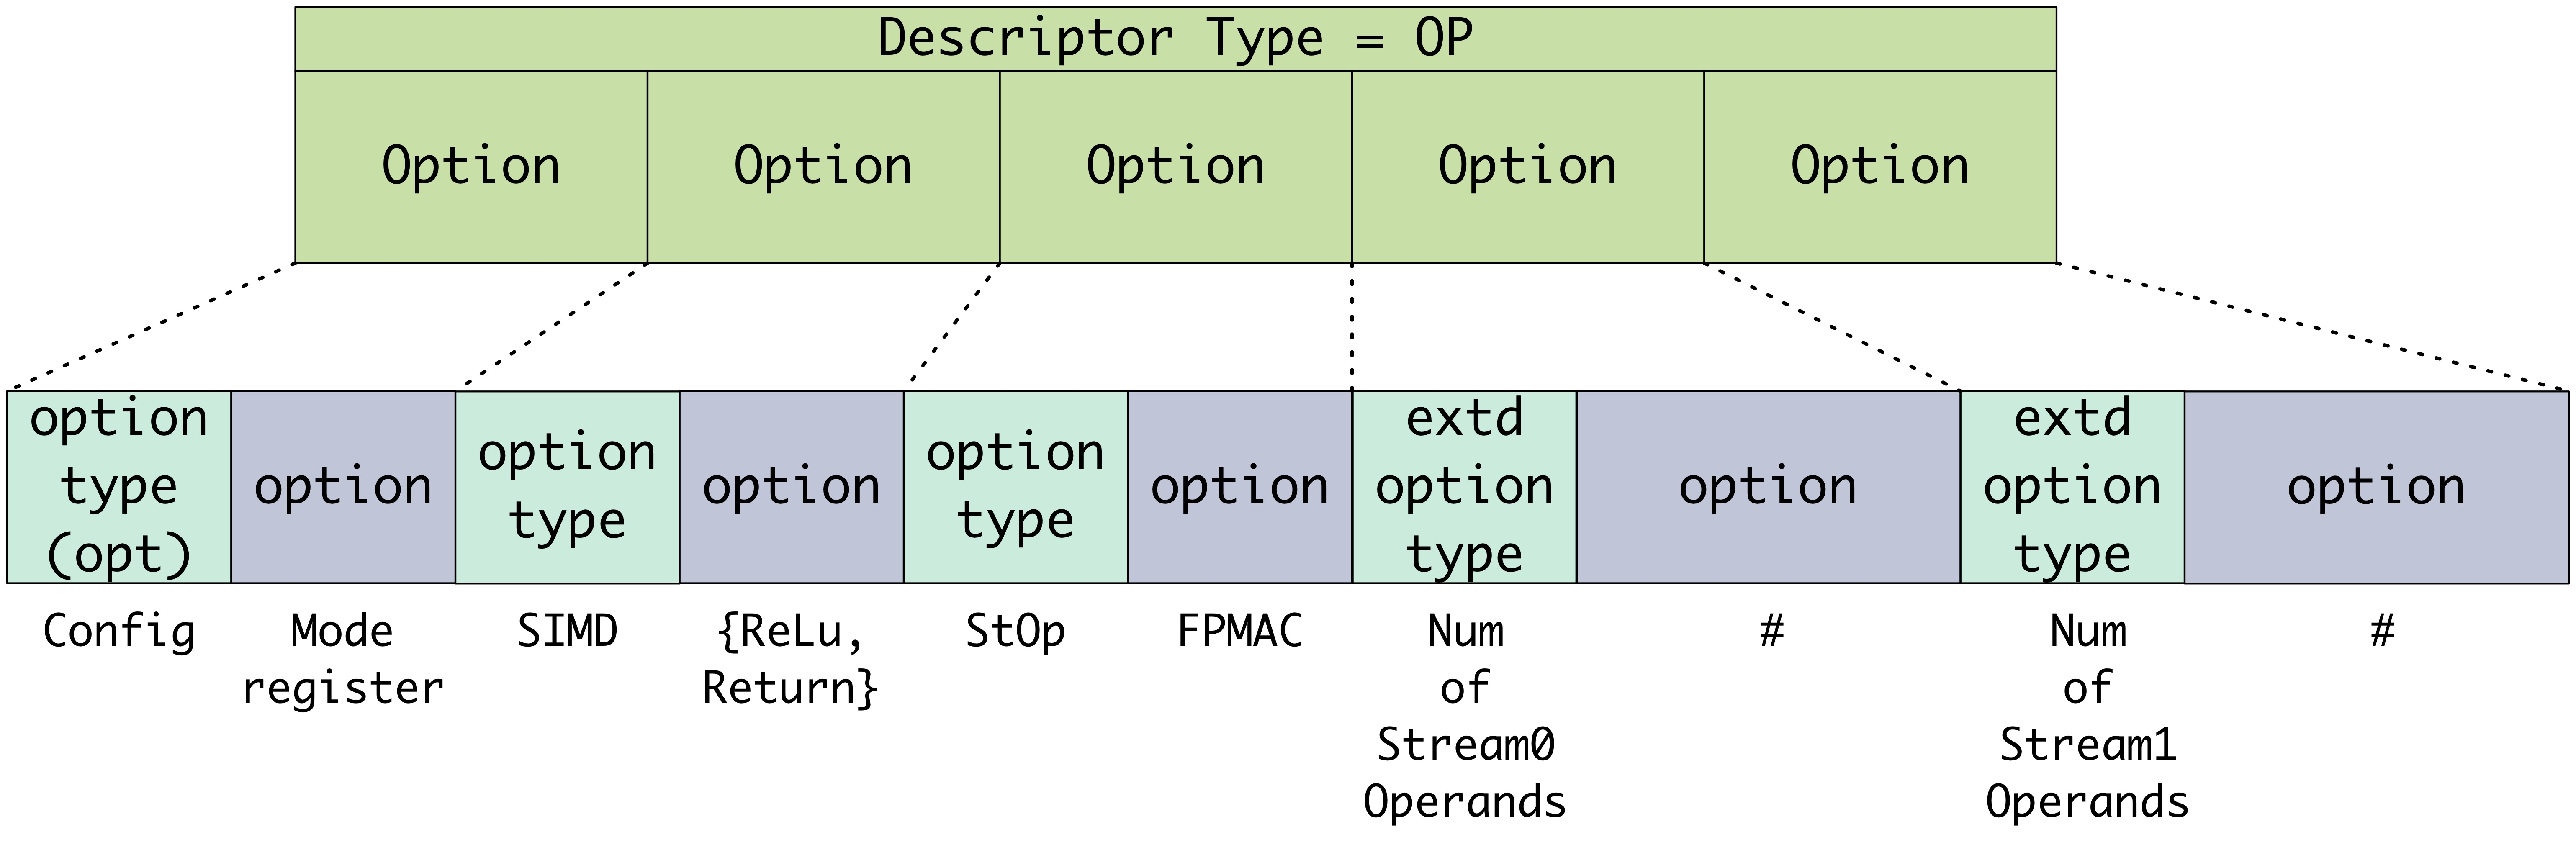
\includegraphics[width=.9\linewidth]{descriptorTuple.jpg}}
}
\caption{Descriptor 6-tuple}
\label{fig:descriptorTuple}
\end{figure}



% ----------------------------------------------------------------------------------------------------
\subsection{Accessing of Pre-synaptic AN states and connection weights}
\label{sec:AccessingANStates}

As was discussed previously, the ANN input and configuration is stored in main \ac{dram} memory. 
A part of the research is determining how to store the ANN input and parameters in such a way to effectively make use of main \ac{dram} bandwidth. 

To provide parameters for the up to 32 execution lanes within the \ac{pe}, the \ac{an} parameters were stored in consecutive address locations. 
With one read to the \ac{dram}, we access 128 words. This provides four weights for each of the 32 ANs being processed. 
These weights are sent to each lane of the \ac{pe} over four cycles. 
We will discuss memory efficiency later, but by taking advantage of the multiple \ac{dram} banks along with pre-fetching and buffering, we are able to achieve relatively high efficiency of the available maximum bandwidth.

Although \ac{an} parameters (weights) are stored in contiguous memory locations, providing the input state to a particular \ac{an} presents us with an interesting problem.

Most often DNNs are represented by layers of ANs whose pre-synaptic neurons are from the previous layer. These previous layers represent the input to a given layer. The first layers input is the actual input to the ANN.


The input can be represented in the form of a 2-D array of AN states. For the sake of generality, the input array elements are considered as AN states.

Any given AN operates on a region of interest (ROI) within the input array.

In figure \ref{fig:roiStorage}, an input to a ANN layer in the form of a 2-D array along with the ROI of two ANs.

\begin{figure}[!t]
\centering
\captionsetup{justification=centering}
\captionsetup{width=.9\linewidth}
\centerline{
\mbox{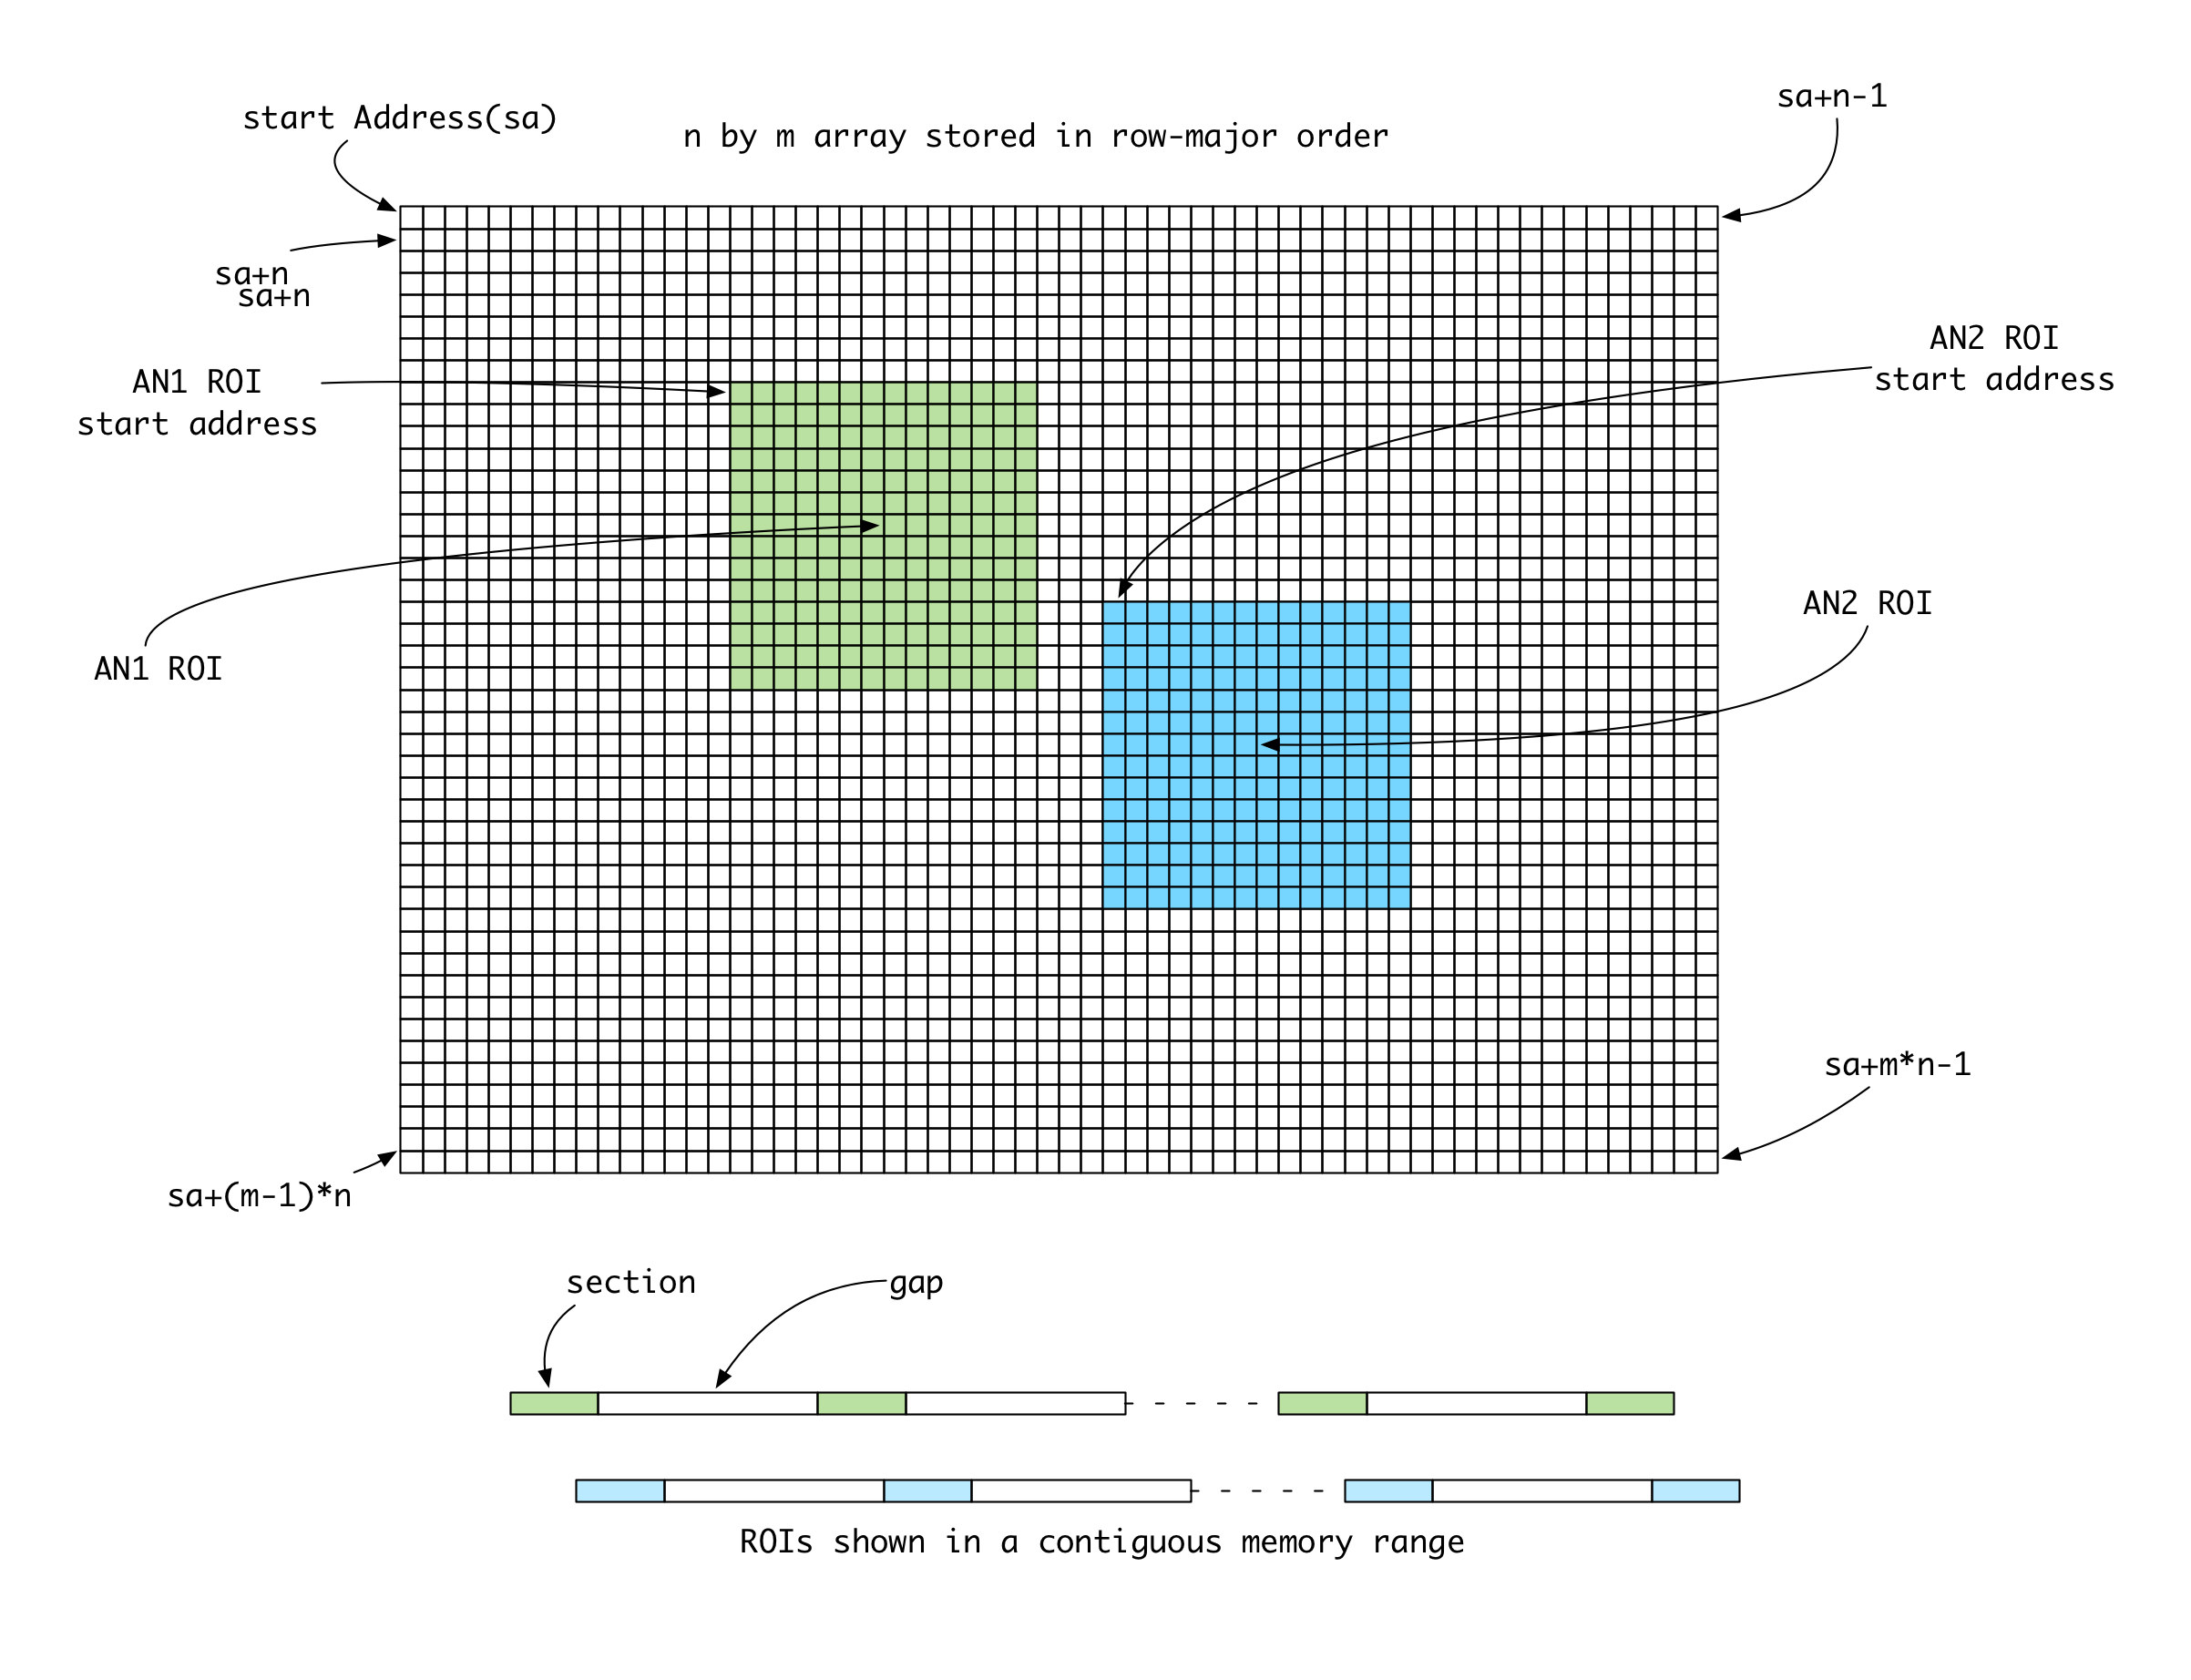
\includegraphics[width=.9\linewidth]{roiStorage.jpg}}
}
\caption{ROI Storage}
\label{fig:roiStorage}
\end{figure}

The various connection weights are stored in multiple contiguous sections. However, its not possible to arrange the input in such a way that each ANs ROI can be stored in contiguous memory locations. The figure above shows a typical ROI arrangement. Assuming the input array is stored in row-major order, an ROI is drawn from disjoint sections of memory. 
These disjoint sections contain a number of AN states and the sections are separated by a gap of a number of memory addresses. When the parameters are accessed when performing a particular operation, the memory controller within the manager must be informed of the start address and the lengths of the sections and gaps. Now this looks problematic, and it is, but in practice groups of ANs share a common ROI. So once we solve the problem of efficiently reading an ROI from the \ac{dram}, that ROI can be shared across a group of ANs

The read efficiency problem is solved by again taking advantage of the \ac{dram}s banks and pages.

This work proposes a data structure to describe these ROI storage locations.

Although disparate groups of ANs may have a different start addresses for their ROI, a commonality is observed in the ROI section lengths and gaps. So for each AN group, the groups ROI starting address is stored along with a pointer to a common set of section length/gaps. This structure is termed a storage descriptor.

This storage descriptor contains, amongst other things the start address of the ROI and a pointer to a section/gap descriptor. Many storage descriptors point to a common section/gap descriptor. This avoids having to have a unique section/gap descriptors for each AN group.

Figure \ref{fig:storageDescriptor} shows the structure of the storage descriptor. The SOD, MOD and EOD are used to delineate each descriptor in memory and stand for start-of-descriptor, middle-of-descriptor and end-of-descriptor.

\begin{figure}[!t]
\centering
\captionsetup{justification=centering}
\captionsetup{width=.9\linewidth}
\centerline{
\mbox{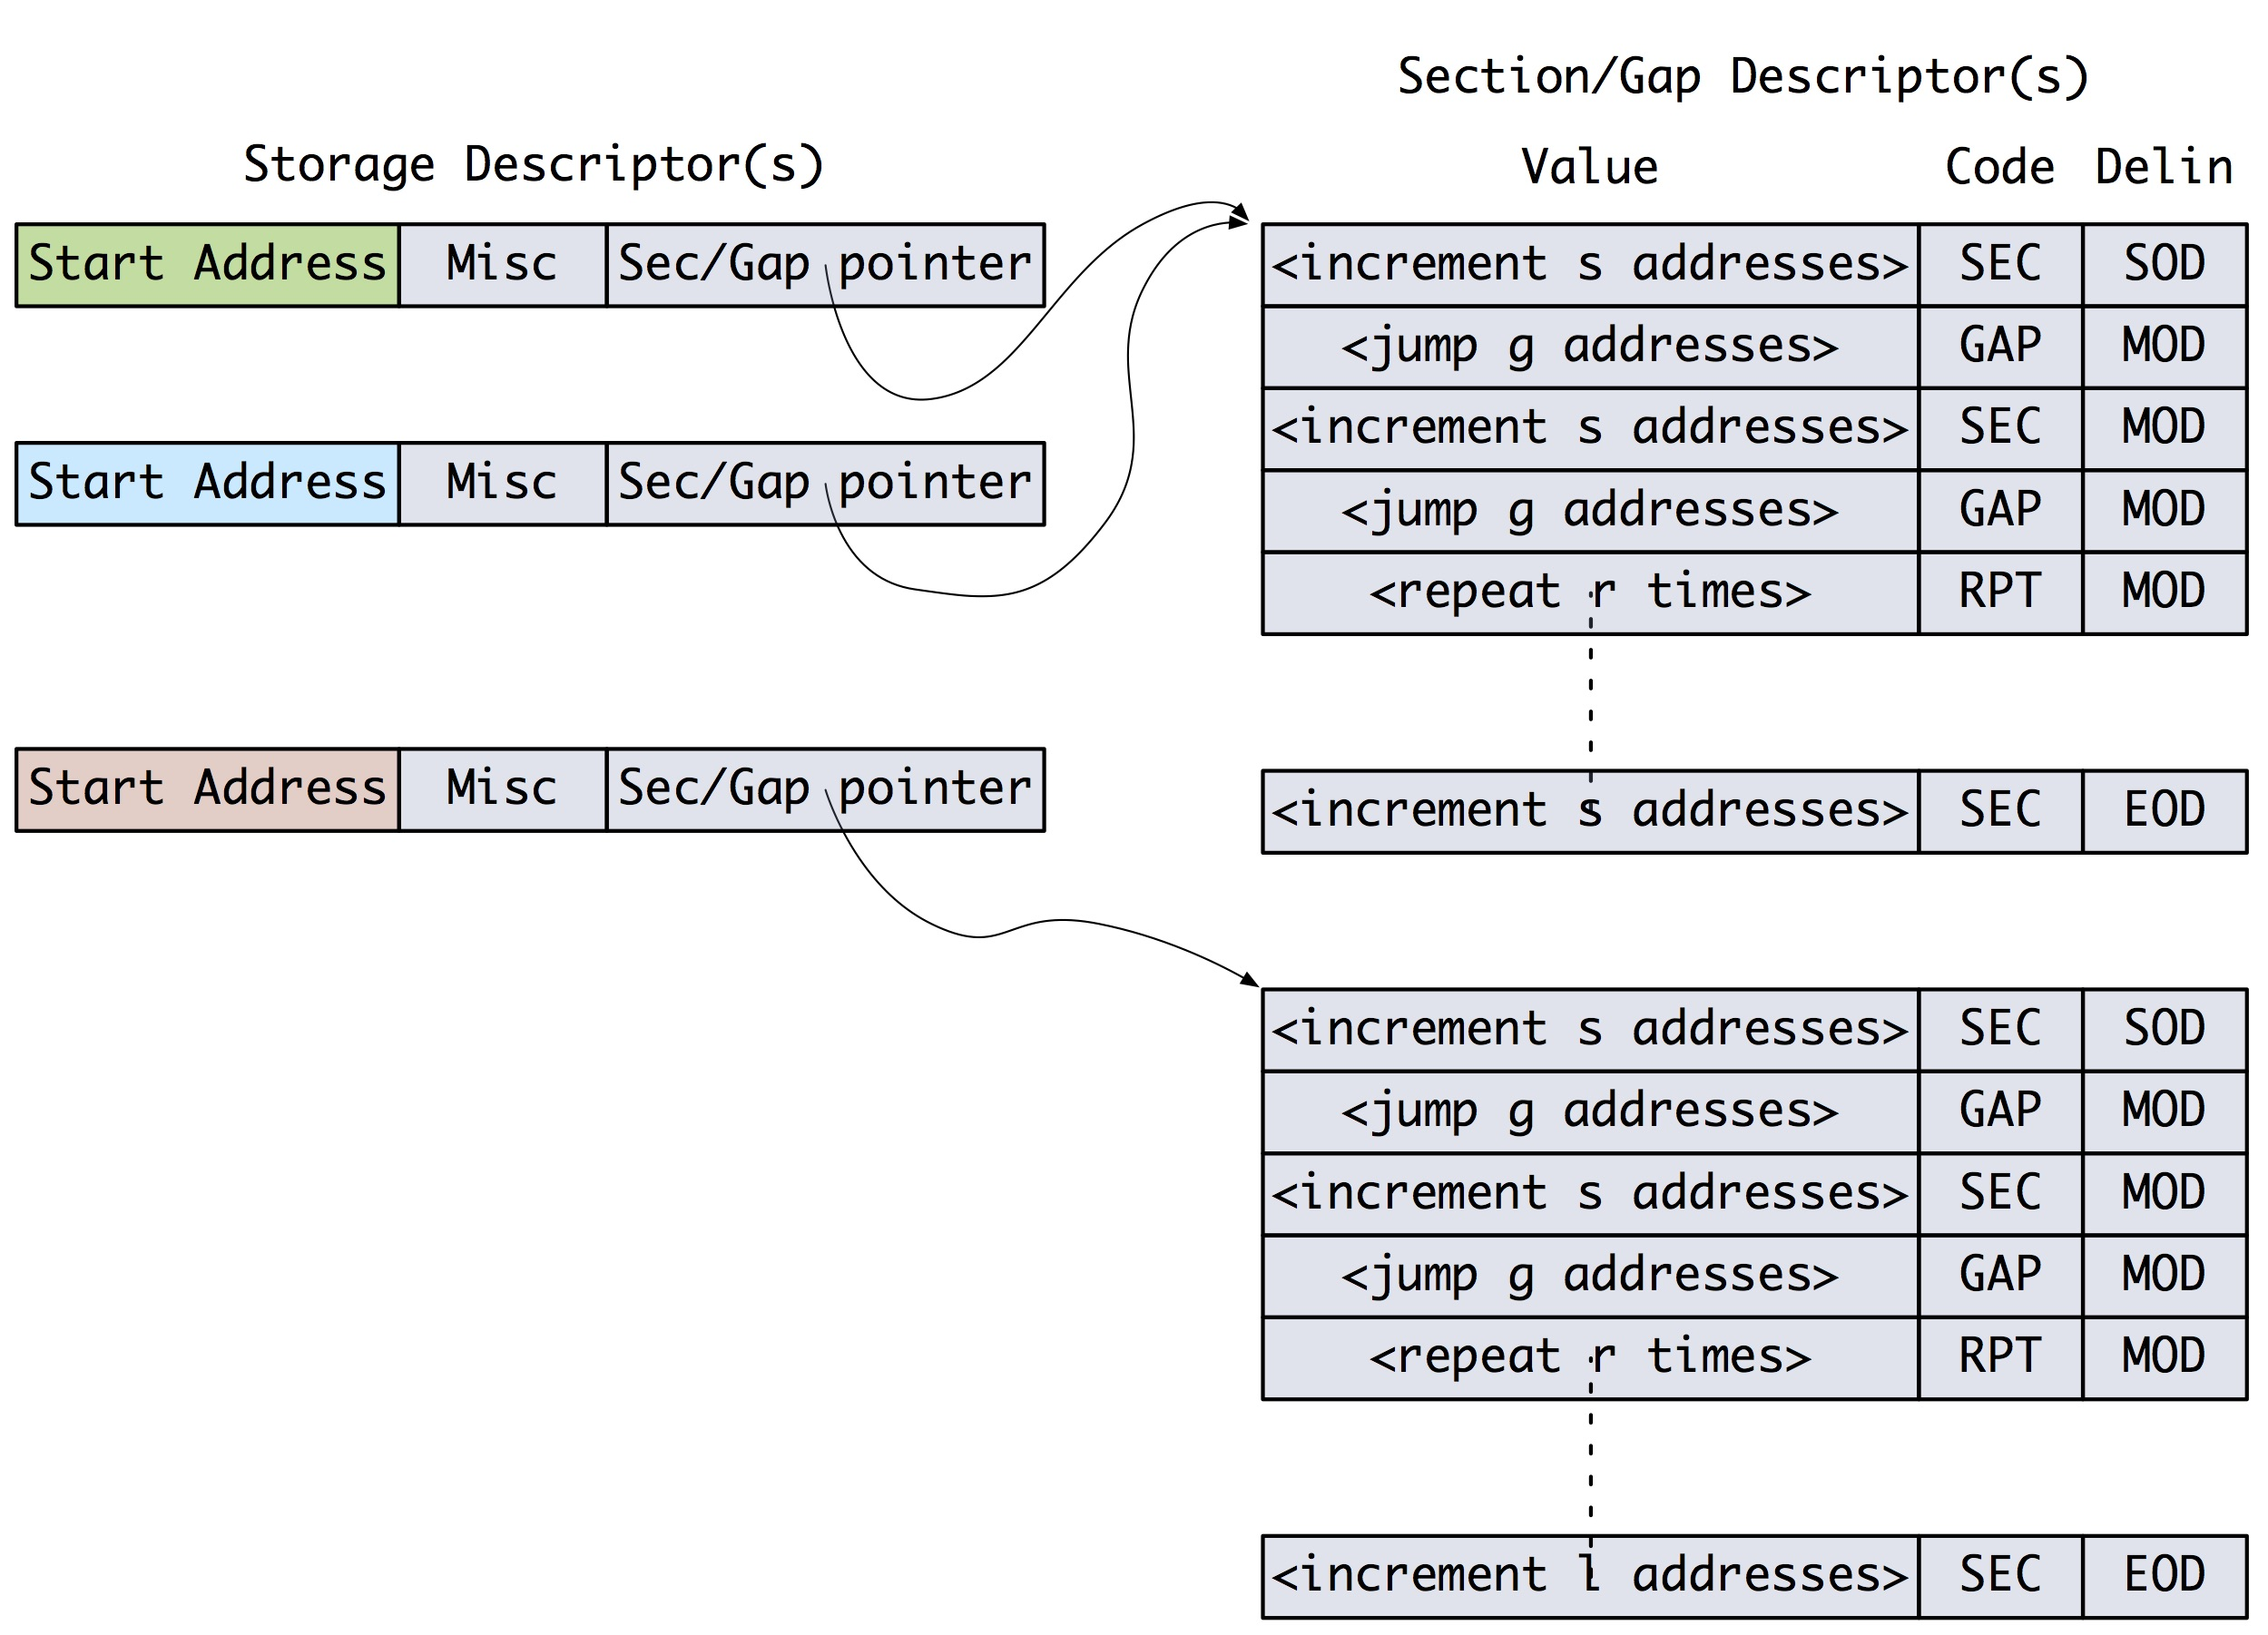
\includegraphics[width=.9\linewidth]{storageDesc.jpg}}
}
\caption{Storage Descriptor}
\label{fig:storageDescriptor}
\end{figure}

% ----------------------------------------------------------------------------------------------------
\subsection{Writing AN state results to memory}
\label{sec:writingANStates}

When the \ac{pe} has processed the group of ANs, the new AN states are sent back to the manager. The manager will store these back to \ac{dram} most likely in the array format as described earlier.

A significant difference taken advantage of is that for any given operation, the system is writing far less than is being read. For example, the ROI and parameters are usually vectors that will typically exceed 100 elements and in many cases much higher. When an operation is complete, in almost all cases one word per lane is writen back to main memory. 
Now that sounds like writing back has a very small impact on performance but with \ac{dram}s thats not always true.

When the system writes the result of an operation back to memory, it is often writing a small portion of a \ac{dram} page and the nature of the \ac{dram} protocol means this is a very inefficient use of \ac{dram} bandwidth. So although the amount of data written is small the performance impact cannot be ignored.

In addition, in many cases the results from a particular \ac{pe} has to be provided not only to the \ac{pe}s local manager but also to other managers. This is handled with a network-on-chip (NoC).

The result storage directives are communicated by using the same storage descriptor mechanism. However, the added complication is because the result will likely have to be replicated to other managers, the storage descriptors must be sent to all destination managers.


% ----------------------------------------------------------------------------------------------------
% ----------------------------------------------------------------------------------------------------
\section{PE Operations}
\label{sec:PE Operations}

% ----------------------------------------------------------------------------------------------------
\subsection{Streaming Operations (\ac{stop})}
\label{sec:streamingOps}
The operations performed by the \ac{stop} are primarily multiple-accumulate with a transfer to the \ac{simd} or to local memory.

Even though the baseline system focuses on the AN multiply-accumulate followed by a ReLu activation function, the system has built in flexibility into the \ac{stop} function to allow other functions to be added

In most cases, the \ac{stop} module will operate on the AN state and weights provided by the manager and provide the result to the \ac{simd}.
% ----------------------------------------------------------------------------------------------------
\subsection{SIMD}
\label{sec:SIMD}

The \ac{simd} is a 32-lane processor with some builtin special functions, such as the ReLu operation.

The \ac{simd} will take the result provided by the \ac{stop} and perform a ReLu. The result will, in most cases, then transmitted back to the manager.

% ----------------------------------------------------------------------------------------------------
\subsection{Configuration}
\label{sec:peConfiguration}

To configure these operations, two pointers are sent to the \ac{pe}. These pointers index into a small local memory which provides a program counter (\ac{pc}) to the function to be performed by the \ac{simd} and a configuration entry for the operation to be performed by the \ac{stop}.

The \ac{pe} is able to perform its operation concurrently on 32-lanes. However, there are cases when less than 32-lanes will be employed. This may occur if the number of ANs being processed is not modulo-32. In this case, the manager provides the number of lanes being processed for any given operation. In addition, the length of the vector of operands is also sent by the manager to the \ac{pe}.




